\section*{EXAMPLES}
In this section, three different examples are discussed. Their purpose is to numerically showcase that our method allows to adaptively refine the mesh to accurately solve an OCP, similarly to ~\cite{Patterson:OCAM:2015}, with the remarkable advantage of an increased computational efficiency for the final enhanced mesh without hindering the accuracy of the final solution. 
%still within the specified tolerance. 
In fact, by allowing to increase the degrees of the approximating polynomials independently for each state, our method effectively adopts to raise them carefully and in a tailored manner. This allows to reduce the overall number of variables of the resulting NLP, with clear benefits in terms of reduced CPU time, memory usage and reduced risk of being trapped by local minima.

Let us now direct our attention to the details. Each problem is transcribed in its initial NLP version by choosing $N = 20$ mesh intervals and by assigning a degree $\dki = 2$ everywhere, i.e. for all $i = 1, \dots, n_x$ and  $k = 1, \dots, N$. The mesh refinement algorithm is then applied with $d_{\min} = 2$, $d_{\max} = 8$ with a prescribed maximum allowable relative error $\epsilon = 1 \cdot 10^{-3}$.

It is worth observing that the $p_{n}h$ and $ph$ tags indicate our mesh refinement method and the one originally proposed by Patterson et al.~\cite{Patterson:OCAM:2015}, respectively.

It is also worth remarking that the final refined mesh for all the three presented examples (both in terms of number and size of $S_{k}$ intervals), turns out to be the same by rolling out both the $p_{n}h$ and the $ph$ approaches. This arises partly as a result that both algorithms share the last section (lines 9-14) of the \emph{Execution} pass in {\bf Algorithm~\ref{alg:step2}}. This means the generic $S_k$ interval is subdivided if and only if at least one state in the generic $S_k$ asks for it.

Each transcribed optimal control problem tested was coded in a scripting environment using the \text{MATLAB} interface to the open-source CasADi framework~\cite{casadi:MPC:2019}.
The CasADi suite can perform AD (Automatic Differentiation) on the code to compute gradients and Jacobians and provides building blocks to efficiently formulate and solve large-scale optimization problems. The back-end solver adopted is IPOPT~\cite{Biegler:CCE:2009} which implements an interior-point algorithm. All the associated NLPs are solved on a laptop with 2.30GHz Intel(R) Core(TM) i7-10875H CPU and 32 GB of RAM.



%%%%%%%%%%%%%%%%%%%%%%%%%%%%%%%%%%%%%%%%%%%%%%%%%%%%%%%%%%%%%%%%%%%%%%
\subsection*{Van Der Pol}
Considering the following optimal control problem namely
driving a \emph{Van der Pol} oscillator to the origin, taken from reference~\cite{casadi:DOC:2018},

\begin{subequations}\label{eq:vanderpol}
	\begin{align}
	\underset{X \in \mathbb{R}^{2}, \, U \in \mathbb{R}}{\text{minimize}}\hspace{8mm}
	&J = \int_{0}^{T}(x_1^{2} + x_2^{2} + u^{2})\,dt  \label{eq:vancost}\\
	\text{subject to} \hspace{8mm}
	& \dot{x}_1 = (1 - x_2^{2})x_{1} - x_2 + u \hspace{5mm} t \in[0,T] \label{eq:vandyn1}\\
	& \dot{x}_2 = x_1 \hspace{28.5mm} t \in[0,T] \label{eq:vandyn2}\\
	& -1  \leq u \leq 1,  \hspace{20mm} t \in[0,T] \label{eq:vanpath1}\\
	& x_2 \geq -0.25,  \hspace{21.5mm} t \in[0,T] \label{eq:vanpath2}\\
	& x_1(0) = 0, \label{eq:initial1}\\		
	& x_2(0) = 1, \label{eq:intial2}		
	\end{align}
\end{subequations}

where $x_1$ and $x_2$ are the two state component (hence $X(t) = [x_1(t), x_2(t)]$), $u$ indicates the element of $U$ (which has dimension $1$), and the dynamics constraints and the initial conditions have been shown explicitly for each state component. In particular, $\dot{X}(t) = [\dot{x}_1(t), \dot{x}_2(t)]$.

In Figs.~\ref{fig:pnh1vanderpol}-\ref{fig:pnh2vanderpol} is shown, for the $\pnh$ algorithm and for the $ph$ one, the final degree of the first state component ($x_1$) and of the second one ($x_2$), respectively. Comparing with the red line, which represents the initial degree, each method increases the states degree. In particular, the green line is equal for the two figures, this means that each state has always the same polynomial degree approximation. Instead, the blue ones are different, hence each state has a different final polynomial approximation. Furthermore, considering the original $S_k$ steps delimited by the dashed gray lines, observing where the green and blue markers increase, it is possible to notice where an $h$-strategy is adopted.
\begin{figure}
	\centering
	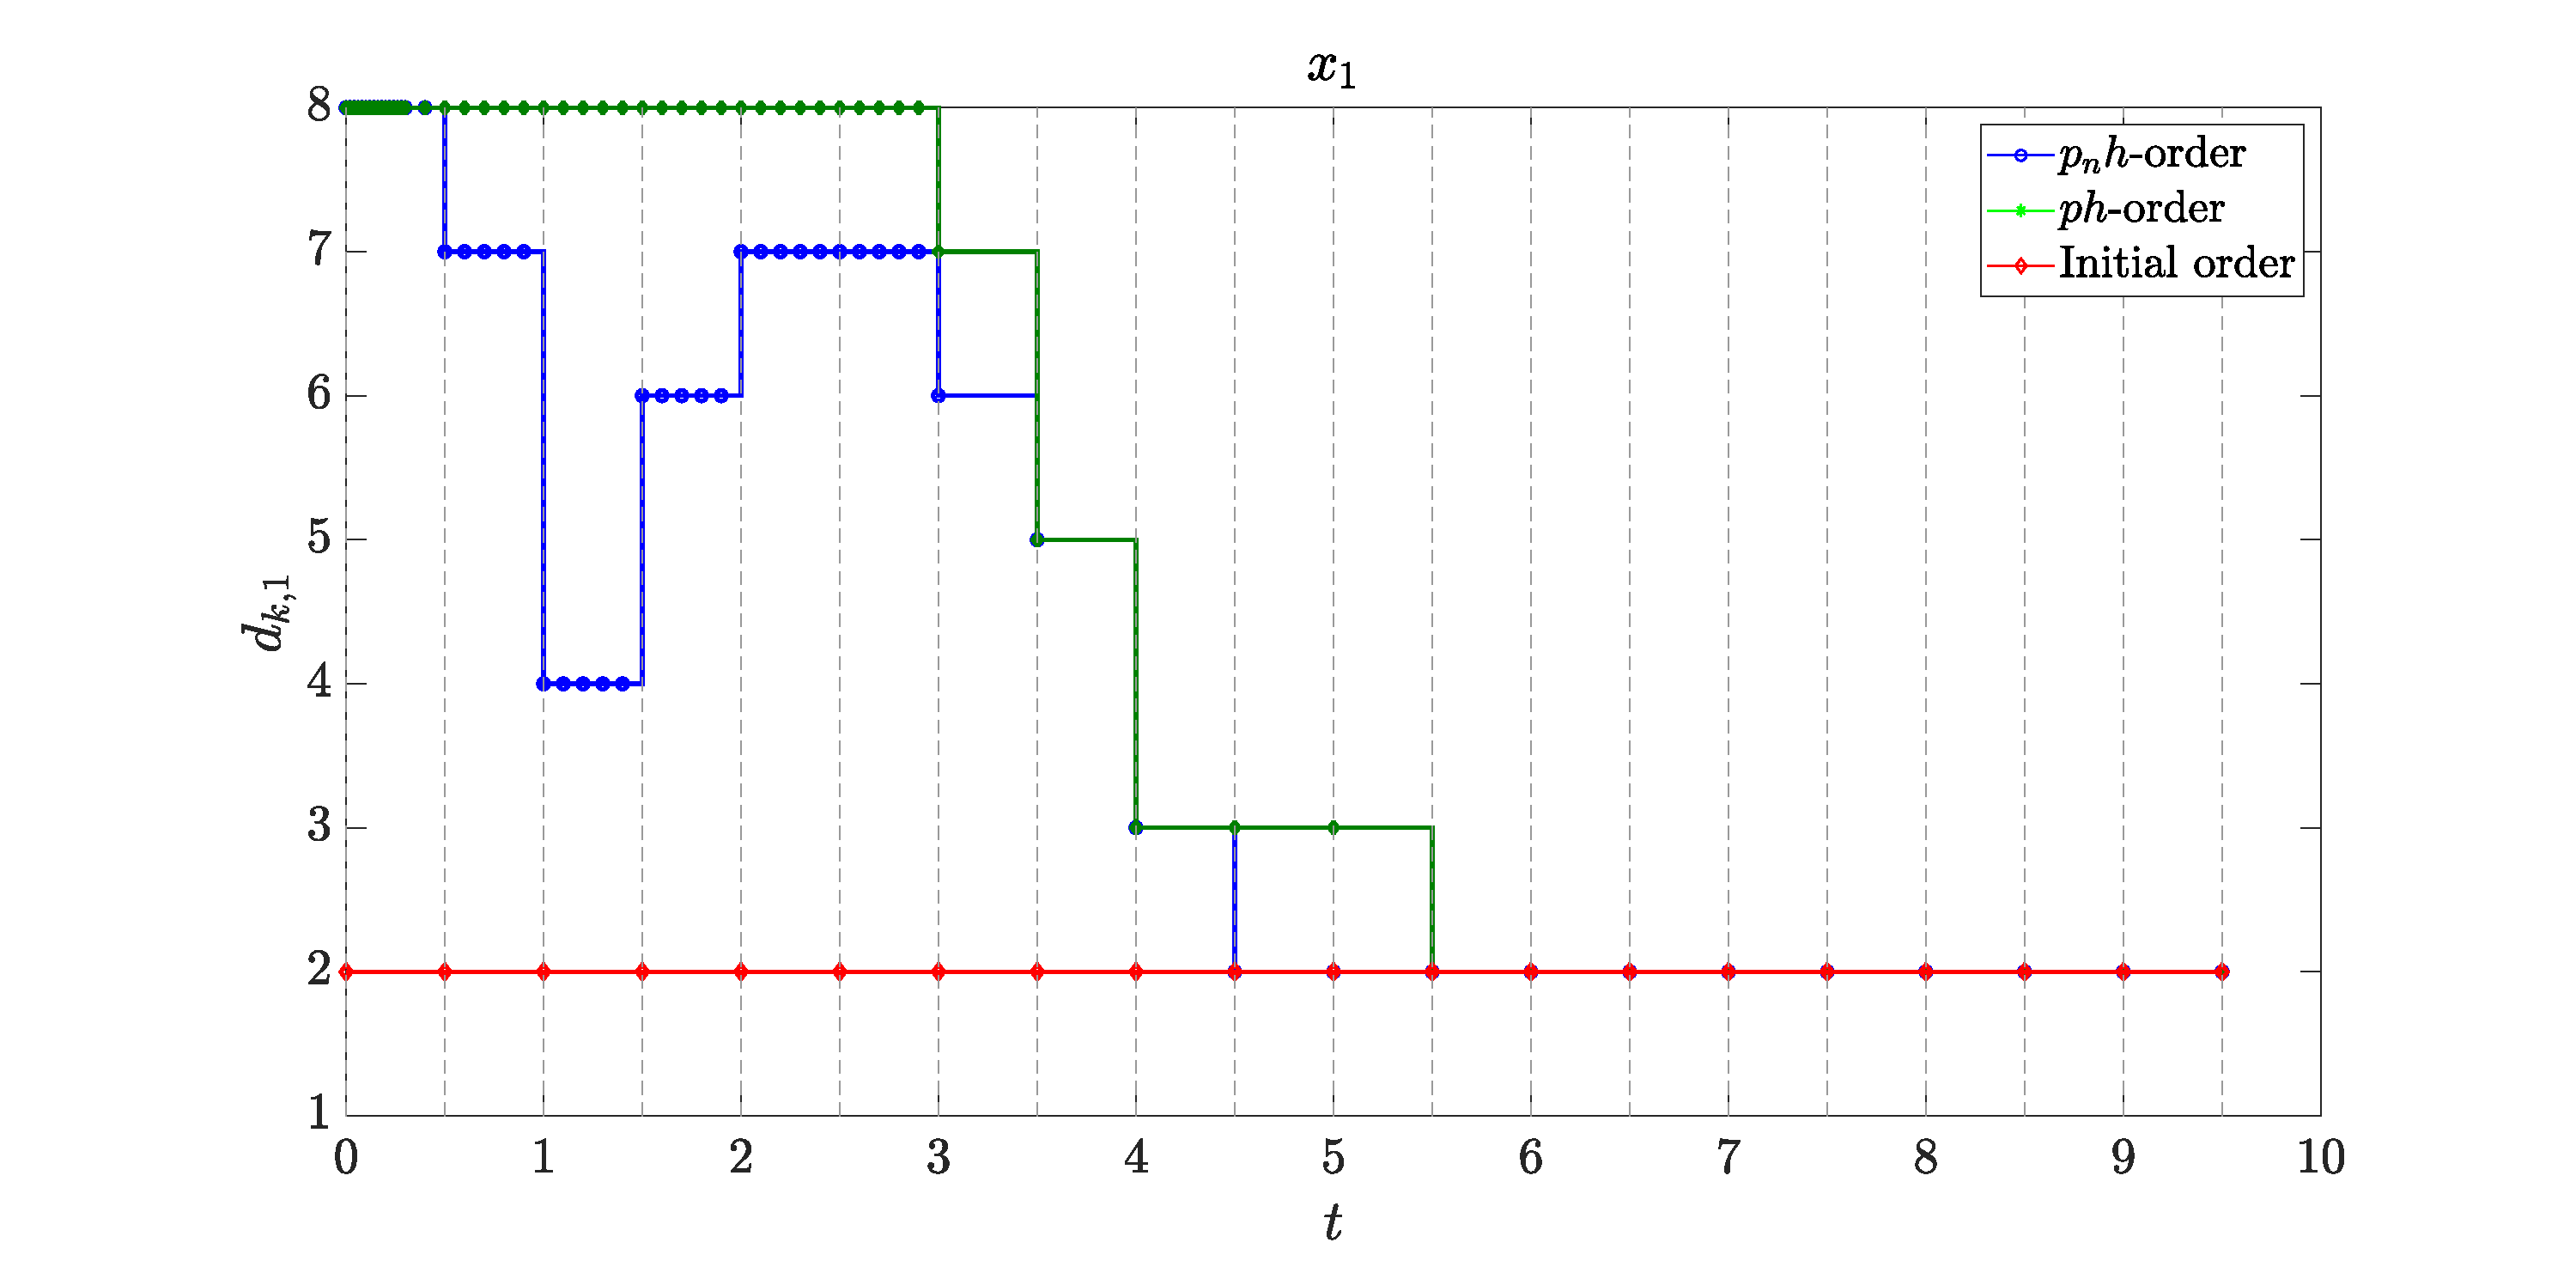
\includegraphics[trim={2cm 0cm 4cm 0cm},clip,width=1.\linewidth]{Img/pnh1_vanderpol}
	\caption{POLYNOMIAL DEGREE OF SECOND STATE ($x_{1}$) FOR THE INITIAL MESH (RED) $\pnh$ ALGORITHM (BLUE) AND $ph$ ALGORITHM (GREEN).}
	\label{fig:pnh1vanderpol}
\end{figure}

\begin{figure}
	\centering
	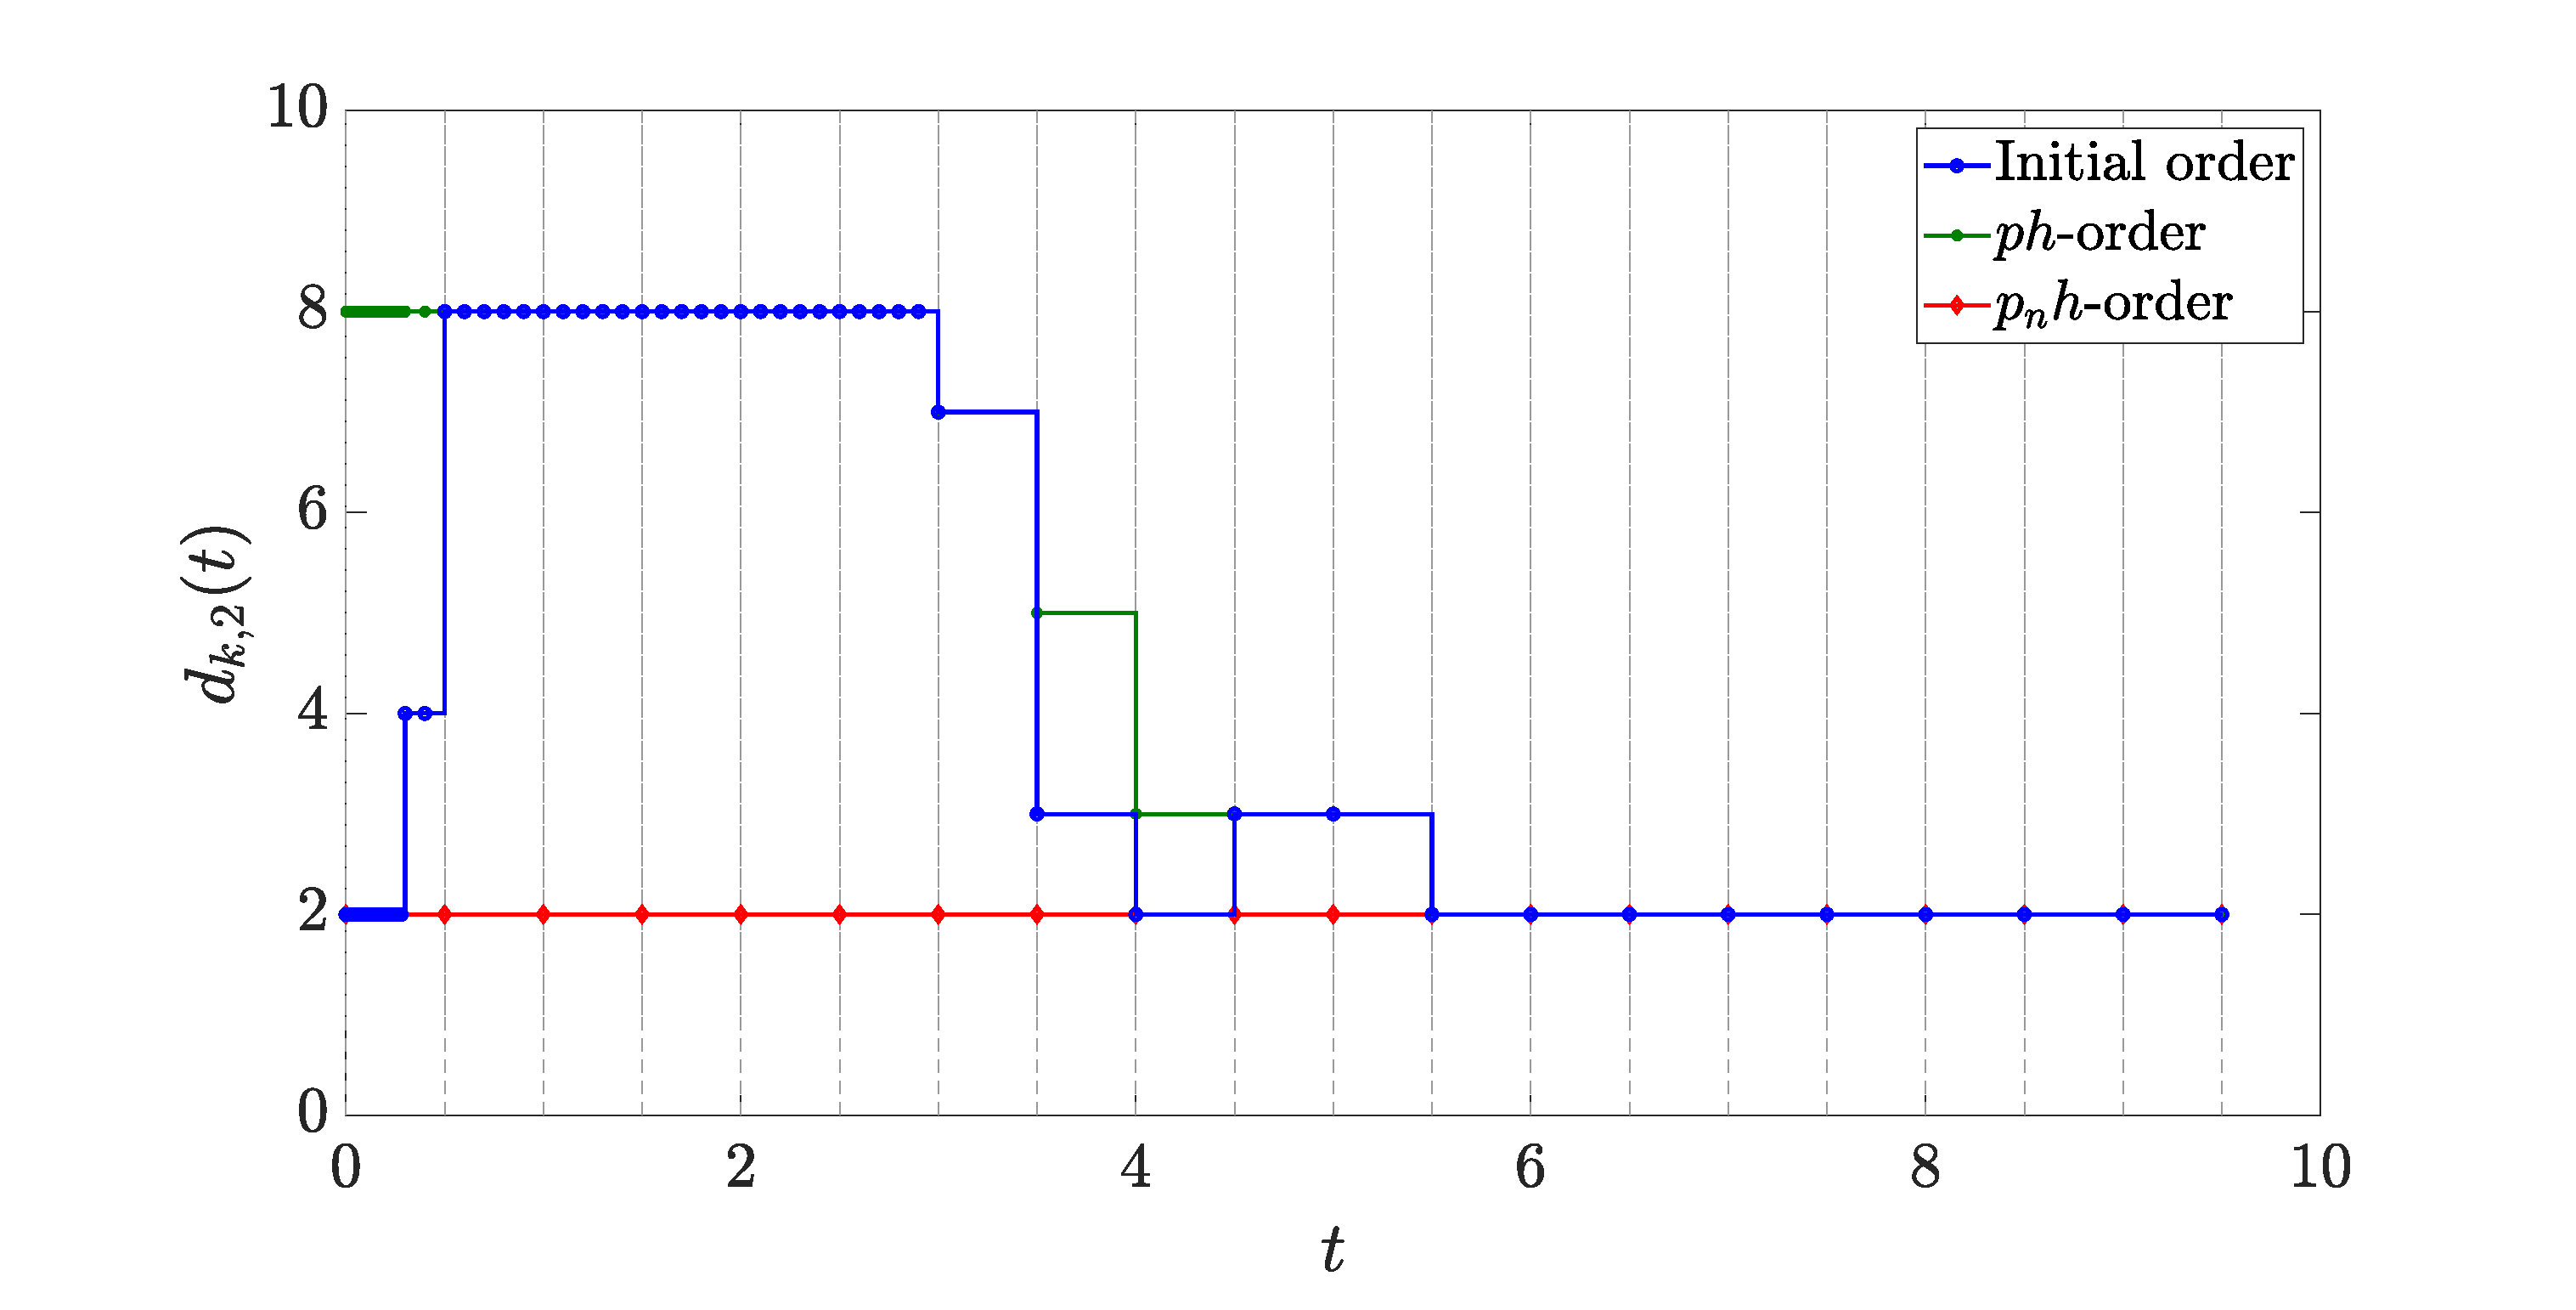
\includegraphics[trim={2cm 0cm 4cm 0cm},clip,width=1.\linewidth]{Img/pnh2_vanderpol}
	\caption{POLYNOMIAL DEGREE OF SECOND STATE ($x_{2}$) FOR THE INITIAL MESH (RED) $\pnh$ ALGORITHM (BLUE) AND $ph$ ALGORITHM (GREEN).}
	\label{fig:pnh2vanderpol}
\end{figure}

In Fig.~\ref{fig:vanderpolstates} the states profile obtained with the $\pnh$ final mesh is shown. In this case the dashed gray lines delimit the final $S_k$ interval. In particular, the nodal values are shown in blue, instead the collocation points in red. That figure shows clearly that the $\pnh$ mesh refinement method places many more collocation and mesh points where the states have greater variations.


\begin{figure}
	\centering
	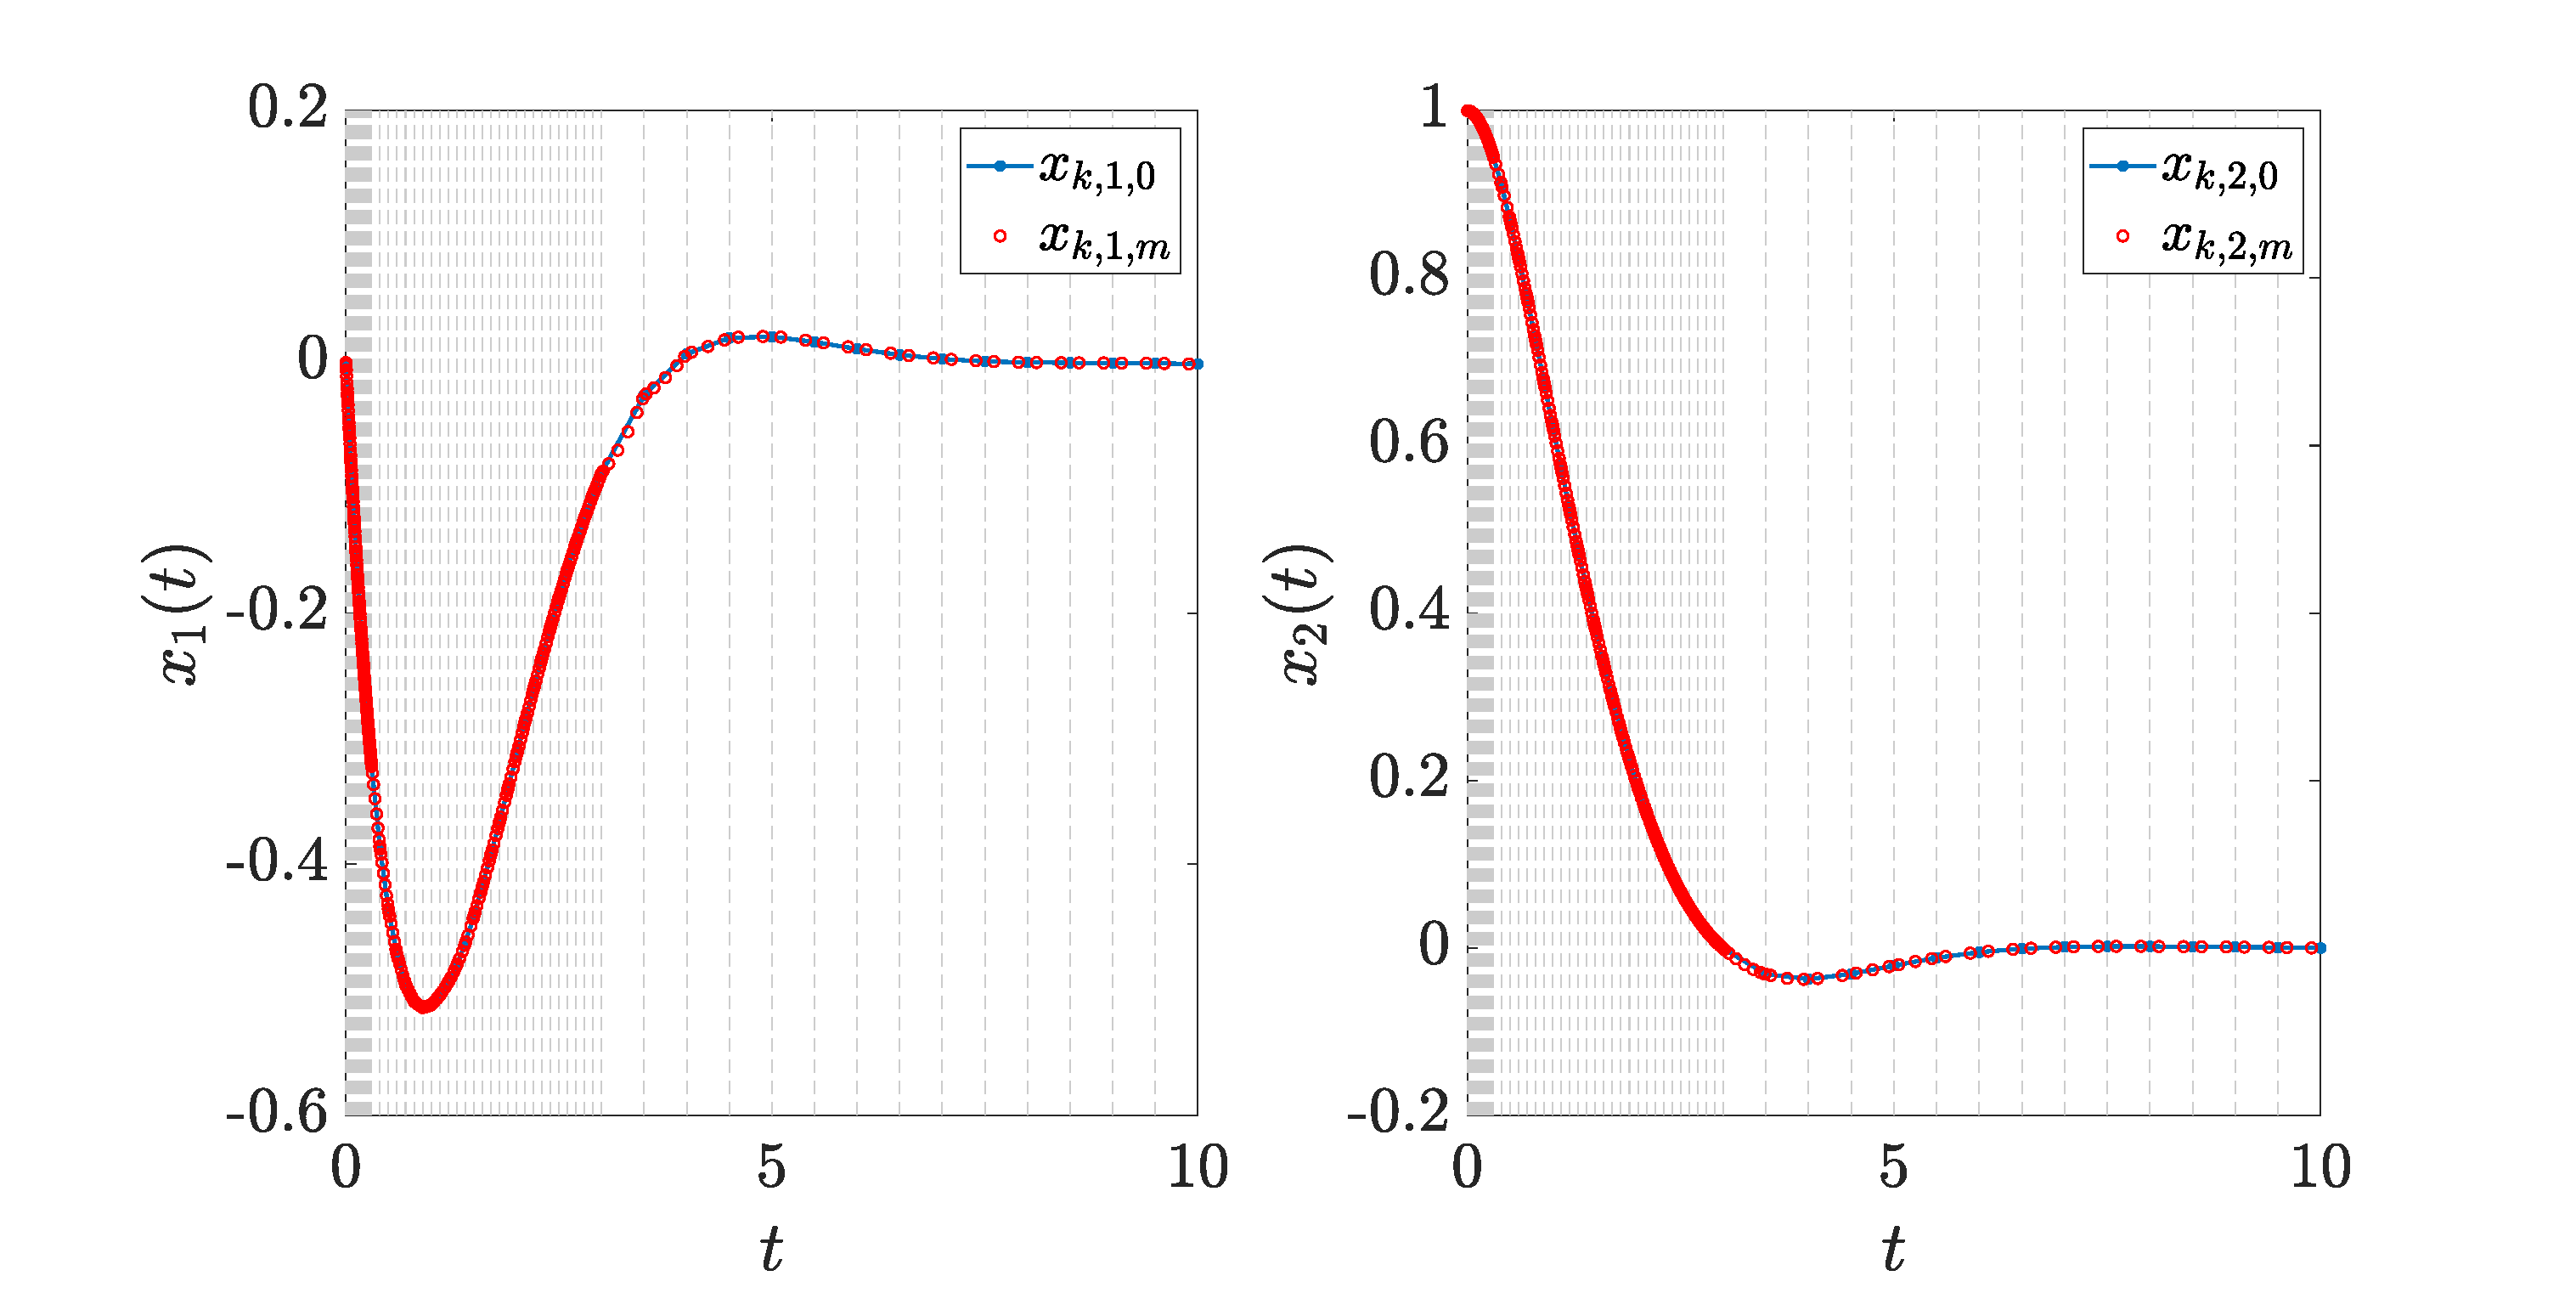
\includegraphics[trim={2cm 0cm 4cm 0cm},clip,width=1.\linewidth]{Img/vanderpol_states}
	\caption{OPTIMAL STATES PROFILE OBTAINED WITH THE $\pnh$ METHOD.}
	\label{fig:vanderpolstates}
\end{figure}

The advantages of the $\pnh$ method, respect to the $ph$ one, are shown in Tab.~\ref{tab:tablevanderpol}, where the column "Mesh" indicates the type of discretization mesh, in particular, "Initial" refers to the initial mesh problem and $ph$ and $\pnh$ refers to the final mesh (hence, the one which guarantees the respect of the $\epsilon$ tolerance), of the~\cite{Patterson:OCAM:2015} and our method, respectively. Then "NLP V." indicates the NLP variables of the resulting discretized OCP problem, "Time NLP" indicates the necessary time to solve the optimal control problem, and "N.I." refers to the number of algorithm iteration necessary to reach the given tolerance. Finally, "Time tot." refers to the total CPU time necessary to reach the imposed convergence criterion, and $e_{max}$  is the maximum of the local error $\ekij$, hence

\begin{equation}
e_{max}= \max\limits_{\substack{j = 1, \dots, \dkip \\ i = 1, \dots, n_x \\ k = 1, \dots, N}} (\ekij)
\end{equation}

\begin{table}[h]
	\caption{FUNDAMENTAL RESULTS QUANTITIES}
	\begin{center}
		\label{tab:tablevanderpol}
		\begin{tabular}{c l l l c c c}
			& & \\ % put some space after the caption
			\hline
			Mesh & NLP V. & Time NLP & N.I. & Time tot. & $e_{max}$ \\
			\hline
			Initial & 140 & 138ms & / & / &  $3.7\mathrm{e}{-2}$\\
			$ph$ & 918 & 500ms & 4 & 23.1s & $9.1\mathrm{e}{-4}$ \\
			$\pnh$ & 769 & 400ms & 4 & 19s & $9.5\mathrm{e}{-4}$ \\
			\hline
		\end{tabular}
	\end{center}
\end{table}

It is worth noting that $\pnh$ method leads to an optimal solution that while respecting the given tolerance $\epsilon$, is obtained from an NLP with fewer variables than $ph$ algorithm.
Hence the final NLP obtained from $\pnh$ method required a lower computational cost and a shorter CPU time.

!!!Figure %%Furthermore considering that $ph$ and $\pnh$ have the same final mesh in terms of $S_k$ number and size, by comparing the solution at the nodal values, the maximum difference between the two solution is for the optimal control $u$.............

\begin{figure}
	\centering
	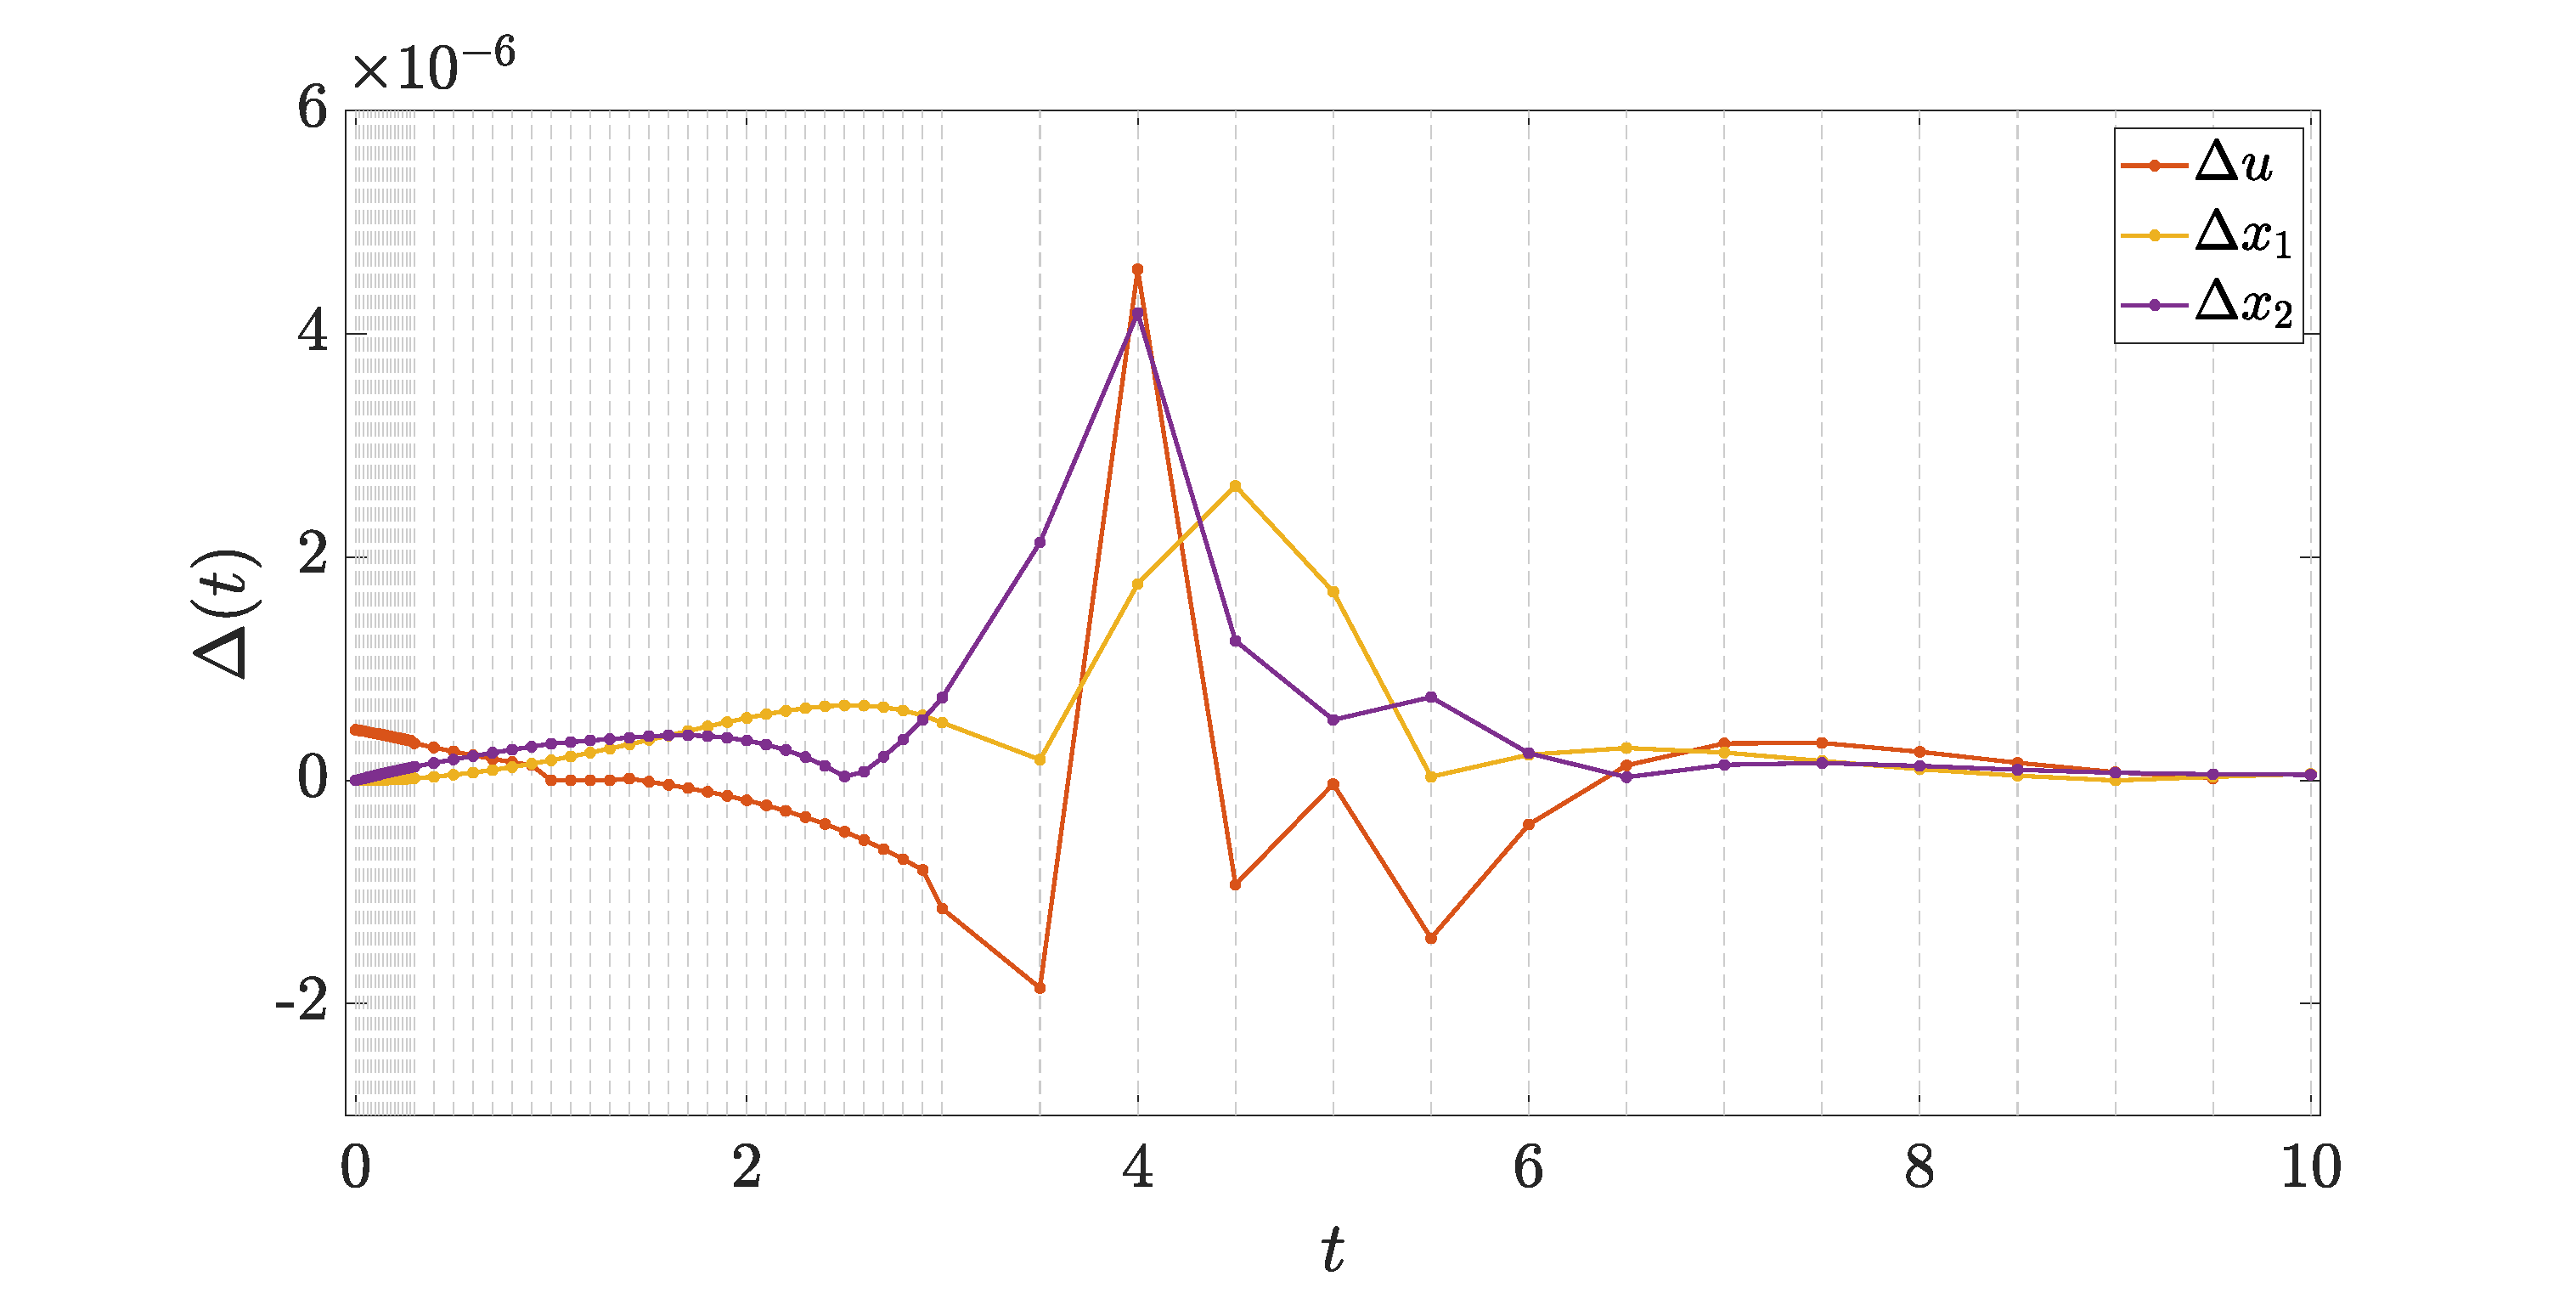
\includegraphics[trim={2cm 0cm 4cm 0cm},clip,width=1.\linewidth]{Img/delta_vanderpol}
	\caption{!!!!!}
	\label{fig:deltavanderpol}
\end{figure}



%%%%%%%%%%%%%%%%%%%%%%%%%%%%%%%%%%%%%%%%%%%%%%%%%%%%%%%%%%%%%%%%%%%%%%
\subsection*{Rolling Disk}
Esempio disco

%%%%%%%%%%%%%%%%%%%%%%%%%%%%%%%%%%%%%%%%%%%%%%%%%%%%%%%%%%%%%%%%%%%%%%
\subsection*{Free Flying Robot}
Esempio free flying robot

%\cite{latex, goosens} 